\section{Training Schedule And Assignments}
\subsection{Training Schedule By Month For The Entire Training Period}
My training schedule is depicted in Table \ref{tab:schedule}. My training schedule is not fixed as there are random task that popped up during my training period.
\begin{table}[h!]
	\caption{Training Schedule}
	\label{tab:schedule}
	\begin{tabularx}{\textwidth}{X|X|X}
		\multicolumn{1}{>{\centering}c|}{\textbf{Task}} & \multicolumn{1}{>{\centering}c|}{\textbf{Metric}} & \multicolumn{1}{c}{\textbf{Month}} \\
		\hline
		Create NLP pipeline to identify conflicts in chatbot dataset & RAM usage and computation time & Jan\\
		Create mockups of dashboard and conduct user testing  & Intuitive designs & Feb\\
		Develop dashboard and integrate NLP pipeline in the backend code & Robustness and latency & Mar\\
		Roll out first version of dashboard on AWS & Robustness and latency & Apr\\
		Setting migration tools and testing on the dashboard & Robustness and accuracy & May\\
		Implement pyspark to handle large training datasets and syncing content between dialogflow and dashboard & Scalability & Jun\\
	\end{tabularx}
\end{table}

\subsection{Training Assignments Completed in 1st Month}
Due to the recent outbreak of Coronavirus in Singapore, my team was tasked to built a chatbot to disseminate information on the Coronavirus situation in Singapore as shown in Figure \ref{fig:govsg-chatbot}. It was done in 2 days. I was involved in training the chatbot on Dialogflow.\\
\noindent
After which, I helped to redesigned the chatbot to give it a more "Telegram" feel. I also scraped information from MOH website to provide end users latest updates on Coronavirus situation in Singapore. Besides, to ensure that adding new training content does not reduce the chatbot's performance, I helped automated regression testing. Test cases are utterances that my team prepare on Google Sheet and the expected response are compared against the actual response obtained from DialogFlow APIs. The automation tool will pull these test cases from Google Sheet, tests the response with Dialogflow APIs, and populated the results back on Google Sheet.
\begin{figure}[h!]
	\begin{center}
		\includegraphics[width=250px]{assets/images/govsg-chatbot.png}
		\caption{GovSG Chatbot To Disseminate Information On nCov}
		\label{fig:govsg-chatbot}
	\end{center}
\end{figure}

\subsection{Training Assignments Completed in 2nd Month}
\noindent
One of my main task is to create a platform to provide end users an overview of the chatbot dataset and identify areas of improvement in the knowledge base. This platform is a web-based dashboard where user only uploads their dataset. After the dataset is processed, the user can go to the dashboard to view and understand the different issues in the chatbot dataset. Before commencing the software development works, I started by doing up mockups using AdobeXD for the dashboard and did user testing to ensure the dashboard is intuitive enough for end user. The mockup for the dashboard page is shown in Figure \ref{fig:aat-dashboard}.

\begin{figure}[h!]
	\begin{center}
		\includegraphics[width=450px]{assets/images/aat-dashboard.png}
		\caption{Mockups for Analytics Dashboard}
		\label{fig:aat-dashboard}
	\end{center}
\end{figure}

\noindent
My second main task was to setup and refine the NLP pipeline. The NLP pipeline is built to identify overlapping intents and ambiguous ones that affect the chatbot performances. I setup BERT and ALBERT to convert text into vectors of numbers (embeddings) that the computer can understand. The embeddings, theoretically, accounts for the semantic meaning. Cosine similarity and hierarchical clustering are performed on these embeddings to identify the problematic intents in the chatbot dataset.

\noindent
As the chatbot dataset can be huge, I optimize one part of NLP pipeline so that the RAM usage will not explode. I also provisioned a AWS EC2 Memory and GPU optimized instances to run my NLP pipeline. 

\noindent
The NLP pipeline helps to identify problematic intents in the training dataset. The source of this problematic intents is mainly a result of end users not understanding that a chatbot cannot handle ambiguous intents. Therefore, training phrases need to be specific. Secondly, end users may not have realized the intents already exist in the training dataset, and added new ones that results in a conflict. Table \ref{tab:nlp-pipeline} shows an example of overlapping intents. My clustering tool in NLP pipeline grouped these set of training phrases together. It is obvious by looking at the training phrases alone, it is difficult to guess the intent. Similarly the chatbot would face the same difficulty that could have resulted in the chatbot's poor performance.

\begin{table}[h!]
	\caption{Sample results of NLP pipeline}
	\label{tab:nlp-pipeline}
	\begin{tabularx}{\textwidth}{X|X}
		\multicolumn{1}{>{\centering}c|}{\textbf{Training Phrases}} & \multicolumn{1}{>{\centering}c}{\textbf{Intents}}\\
		\hline
		Tax reference No Fxxx & How do I contact IRAS? \\
		ref no Fxxx & GPF 58 What is the User ID? What is my tax reference number?\\
		Tax reference no Gxxx & What is the User ID?\\
	\end{tabularx}
\end{table}
\subsection{Training Assignments Completed in 3rd Month}
\noindent
One task I did was Topic Modeling. I use Gensim and Mallet to identify topics in positive and negative sentiments. These topic helped Product Owners understand the strength and weakness of current digital products for areas of improvements. A sample result of the topic modeling for negative sentiment is show in Table \ref{tab:topic-modeling}.

\begin{table}[h!]
	\caption{Sample results of topic modeling}
	\label{tab:topic-modeling}
	\begin{tabularx}{\textwidth}{X|X|X}
		\multicolumn{1}{>{\centering}c|}{\textbf{Topic}} & \multicolumn{1}{>{\centering}c|}{\textbf{Keywords}} & \multicolumn{1}{c}{\textbf{Text}} \\
		\hline
		1 & card, credit, detail, key, info, save, store, scan, regular, future & 
		Re-input of credit card payment details each time. Maybe ca scan or take photo of credit card to capture details or save last transaction details.\\
		2 & card, detail, credit, key, remember, input, type, everytime, color, product & Remember my credit card number except my ccv number expiry date. At least I can input my card number w/o going to wallet downstairs to key in again.\\
	\end{tabularx}
\end{table}

\noindent
Topic modeling identifies a set of most representative keywords that could help Product Owners deduce the topic. I also find the most representative sentiment for each topic to provide context to these keywords. For example, Topic 1 in Table \ref{tab:topic-modeling} suggests caching of user details so that user does not have to re-input the same details subsequently.

\noindent
Another task I completed was to setup the backend code in Flask for the analytics dashboard. All the endpoints for the backend have been exposed. Sentry is setup to monitor for errors during runtime. PyTest was setup for unit and integration test. SwaggerHub was also setup for document the RestAPIs. RQ and Redis was also setup for the queuing system to run long computation tasks in the background. MongoDB was also setup to store results in the NLP pipeline. The backend code is also dockerized and deployed on AWS.

\subsection{Training Assignments Completed in 4th Month}
\noindent
One task I completed was to deploy the application on Kubernetes using AWS EKS. The finished product on the staging environment is shown in Figure \ref{fig:aat-staging}. There were some modications made to the UI to make the dashboard more user friendly and intuitive. The application is deployed on Kubernetes to orchestrate the various Dockers to run the application. I also setup the Kubernetes dashboard to visualize the different resources and services in my Kubernetes cluster. Kubernetes has also help me to scale up and down resources base on the traffic, and update and deploy new images. 

\begin{figure}[h!]
	\begin{center}
		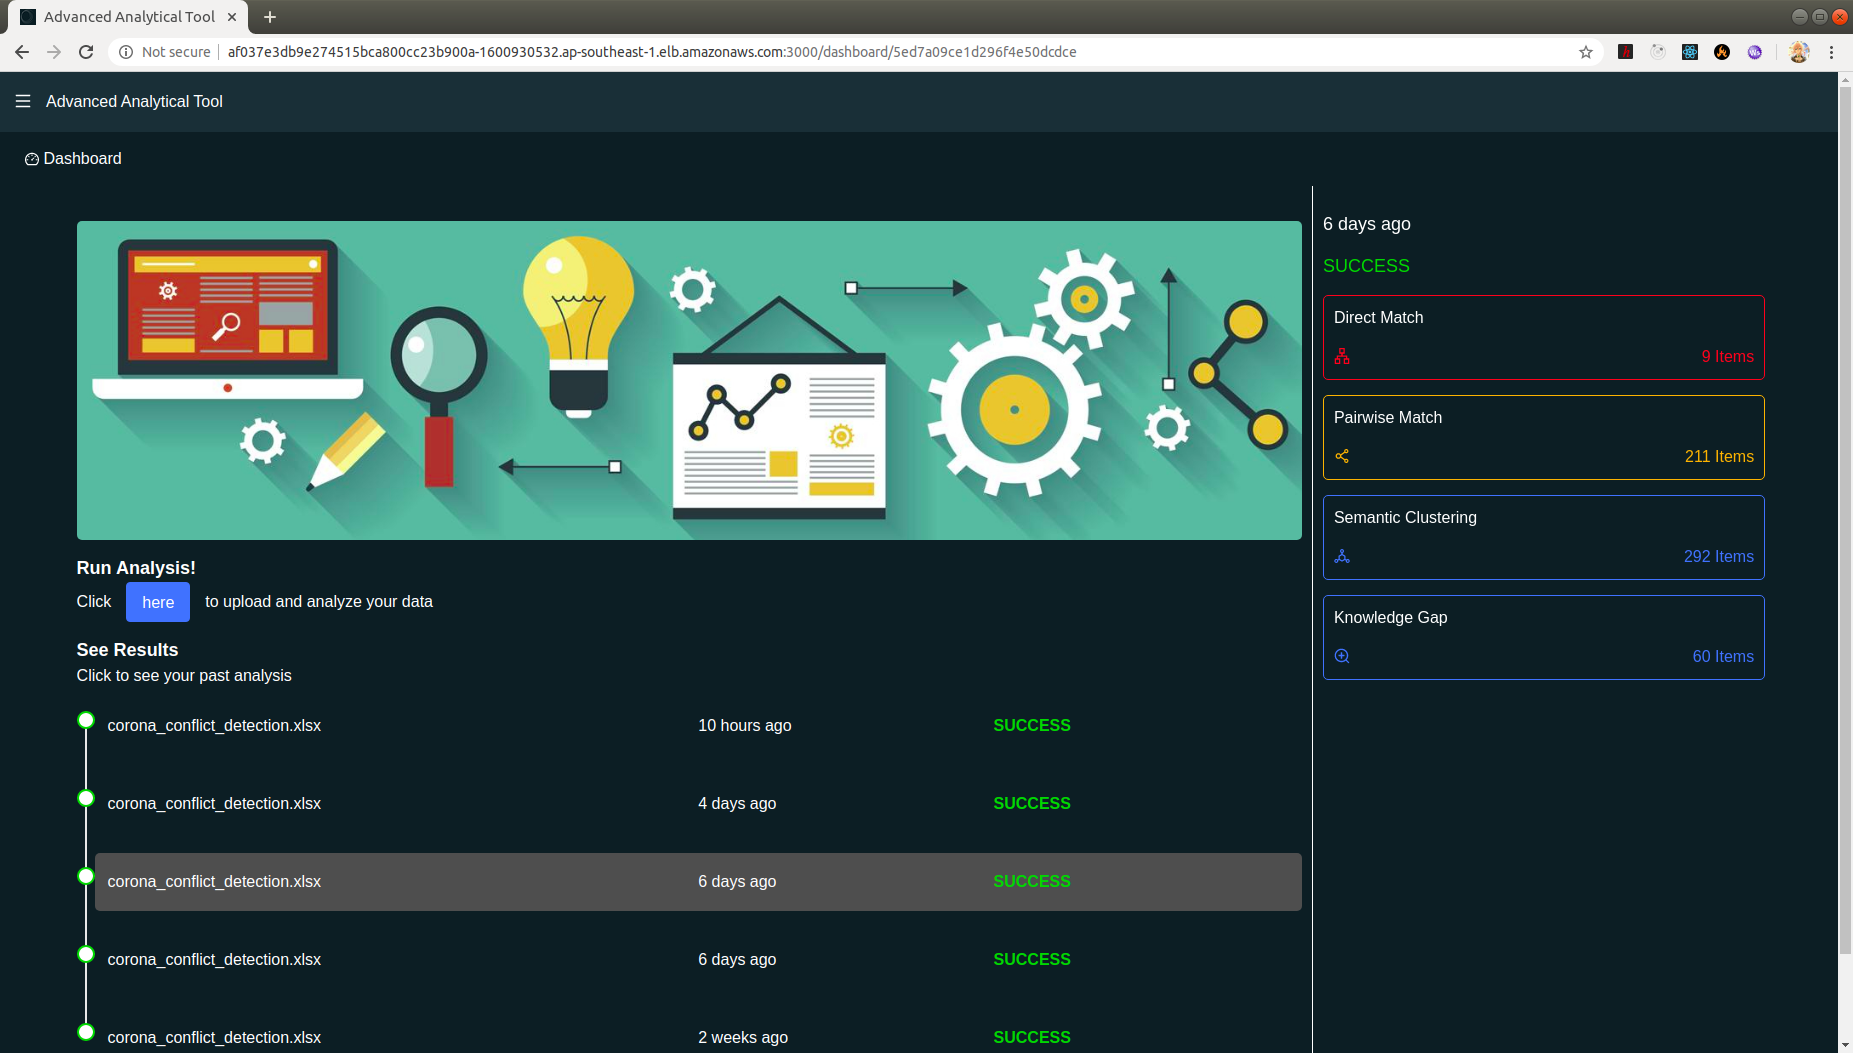
\includegraphics[width=450px]{assets/images/aat-staging.png}
		\caption{Dashboard on Staging Environemnt}
		\label{fig:aat-staging}
	\end{center}
\end{figure}

\noindent
Another tasks I completed was to setup the regression test using Docker Compose. This allows the integration and unit testing to be containerized so that system requirements and dependencies are tested on the same environment as production's during continuous integration. To determine whether continuous integration is successful, the image for testing is built and run. The exit status of the image after the test is finish is listened to determine whether all tests passed or not.

\subsection{Training Assignments Completed in 5th Month}
\noindent
One task I did was to develop the APIs to allow users to migrate the training dataset from FlexAnswer to DialogFlow. The way the data are stored in both platforms are different, and requires some data structures and algorithms, such as Breath First Search and Depth First Search, to group the training dataset into the correct parts of a conversation flow. Besides, there are many edge cases due to poor integrity of the dataset or missing values. Currently, the user first need to upload their DialogFlow chatbot's credentials on the dashboard, shown in \ref{fig:aat-agents}, to later upload and migrate the data from FlexAnswer to DialogFlow.

\begin{figure}[h!]
	\begin{center}
		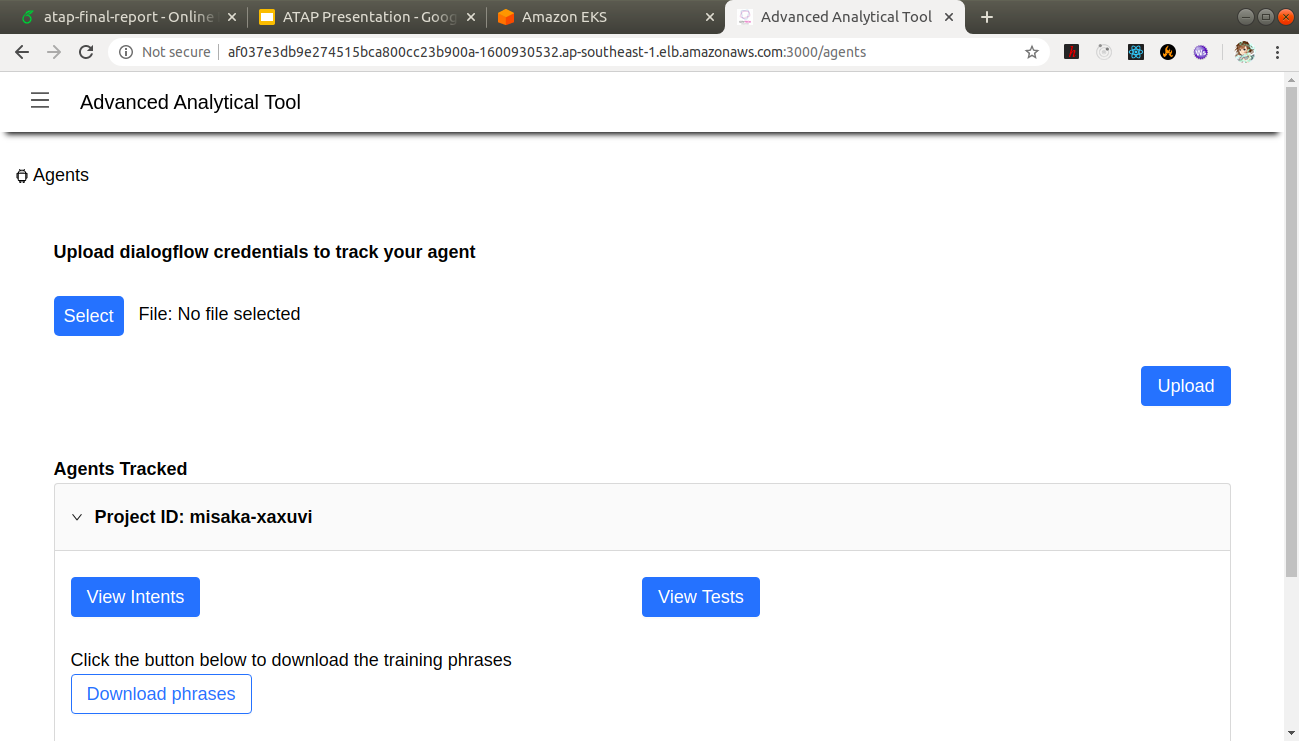
\includegraphics[width=450px]{assets/images/aat-agents.png}
		\caption{Agents Page in Dashboard}
		\label{fig:aat-agents}
	\end{center}
\end{figure}

\noindent
Another tasks I completed was to setup logging on both the frontend and backend. I used the AWS CloudWatch to log the messages from both frontend and backend to. I found interested libraries, such as winston-cloudwatch for frontend and watchtower for backend to convinently setup a queue system to log the messages without encountering conflicts. The logging had helped one of the team member to debug the deployment error with Nginx which rejects headers with underscores. 

\subsection{Training Assignments Completed in 6th Month}
\noindent
One task I did was to build a scalable pipeline that provides the same analysis as the pipeline that I deployed to the Kubernetes cluster. PySpark allows the memory consumed to be distributed; therefore, the analysis can be scalable. I used SparkNLP to extract out the embeddings and performs KMeans with the distance metrics as cosine similarity. The scalable pipeline download the files from AWS S3, reads the dataset, performs similar analyses, and then uploads the files back to AWS S3. The only difference is that it is using PySpark for scalability.

\noindent
Another tasks I completed was to implement APIs to perform CRUD on the intents, training phrases, entities, and responses. Last month, I made a similar attempt for the intents and training phrases; however, the approach is not production ready and stable. The current changes made is to mark items deleted with a boolean flag instead of actually deleting the item. Secondly, the training phrases are stored a string without its entities. I made the changes to the implementation to support storage of the training phrases with entities.